% !TEX program = lualatex
\documentclass[a4paper,11pt]{bxjsarticle}
%
% fontsetup-noto.tex (simple + robust)
\usepackage{luatexja}
\usepackage{luatexja-fontspec}
\usepackage{fontspec}

% Japanese + Latin: use CJK fonts (they include Latin glyphs)
\setmainfont{Noto Serif CJK JP}
\setsansfont{Noto Sans CJK JP}

\setmainjfont{Noto Serif CJK JP}
\setsansjfont{Noto Sans CJK JP}

% Mono: try Noto Sans Mono, fallback to Latin Modern Mono
\IfFontExistsTF{Noto Sans Mono}{
  \setmonofont{Noto Sans Mono}[Scale=MatchLowercase]
}{
  \setmonofont{Latin Modern Mono}[Scale=MatchLowercase]
}

%% fontsetup-harano.tex
% Use HaranoAji (bundled with TeX Live Japanese collections)
\usepackage{luatexja}
\usepackage{luatexja-fontspec}
\usepackage{fontspec}

% Select by FILE NAME to avoid HaranoAji*.fontspec auto-weight requests.
\setmainjfont{HaranoAjiMincho-Regular.otf}[
  Path=fonts/,
  BoldFont=HaranoAjiMincho-Bold.otf
]
\setsansjfont{HaranoAjiGothic-Regular.otf}[
  Path=fonts/,
  BoldFont=HaranoAjiGothic-Bold.otf
]

% Latin / mono
\setmainfont{Latin Modern Roman}
\setsansfont{Latin Modern Sans}
\setmonofont{Latin Modern Mono}[Scale=MatchLowercase]

%\usepackage{luatexja}
\usepackage{luatexja-fontspec}

\setmainjfont{HaranoAjiMincho}[
  BoldFont = HaranoAjiMincho-Bold
]
\setsansjfont{HaranoAjiGothic}[
  BoldFont = HaranoAjiGothic-Bold
]


% ===== Heading control =====
\usepackage{titlesec}
% 見出しだけゴシック太字(和文=gtfamily, 欧文=sffamily)
\titleformat{\section}
  {\sffamily\gtfamily\Large\bfseries}
  {\thesection}{1em}{}
\titleformat{\subsection}
  {\sffamily\gtfamily\large\bfseries}
  {\thesubsection}{1em}{}
\titleformat{\subsubsection}
  {\sffamily\gtfamily\normalsize\bfseries}
  {\thesubsubsection}{1em}{}  
% 段落字下げ(1zw相当)
\setlength{\parindent}{1em}
% 字間(luatexja)
%\ltjsetparameter{
%  kanjiskip = {0pt plus 0.4pt minus 0.5pt},
%  xkanjiskip = {0.20em plus 0.15em minus 0.06em}
%}
\ltjsetparameter{
  kanjiskip  = {0pt plus 0.4pt minus 0.5pt},
  xkanjiskip = {0.20em plus 0.10em minus 0.05em}
}
% ---- 行間:詰まり/広がりを最後に微調整 ----
 \linespread{1.00}  % まず 1.00 / 1.03 / 1.06 を比較

  
\usepackage{geometry}
\geometry{a4paper,margin=18mm}
\usepackage{amsmath,amssymb}
\usepackage{graphicx}
\usepackage{hyperref}
\usepackage{siunitx}
\usepackage{bm}
\usepackage{booktabs}
\usepackage{longtable}
\usepackage{xcolor}
\usepackage{listings}
\usepackage{caption}
\usepackage{enumitem}
\usepackage{float} %
\usepackage{subcaption}
\captionsetup[subfigure]{
    position=top,
    justification=raggedright, % 左寄せ
    singlelinecheck=off        % キャプションが短くても左寄せを維持する
}

\lstset{
  basicstyle=\ttfamily\footnotesize,
  columns=fullflexible,
  breaklines=true,
  frame=single,
  framerule=0.4pt,
  numbers=left,
  numberstyle=\tiny,
  xleftmargin=2.2em,
  showstringspaces=false
}

\title{IPSモード液晶の光学補償偏光板の最適化設計思想}
\author{
BOE Varitronix Japan\\  
坂本 道昭
}
\date{\today}

\begin{document}
%
\maketitle
%
\begin{abstract}
IPS(In-Plane Switching)モード液晶において,暗状態での斜入射観察時に生じる光漏れは,
とくに対角方向の視野角で顕著となり,コントラスト比(CR)の劣化を引き起こす主要因である.
この現象は,出射偏光板(Analyzer)の有効透過軸が斜入射により回転し,正面では成立していた
入射偏光板(Polarizer)と出射偏光板(Analyzer)のクロスニコル条件が斜め視点(オフアクシス)
で破綻することに起因する.

本研究では,液晶層および A-plate,C-plate などの光学補償板を含む光学セルを対象とし,
斜入射における有効偏光軸回転と角度依存リタデーションを厳密に取り込んだ数値モデルを構築した.
伝搬方向に直交する横波面上で定義した有効 Jones 伝達演算子を用いて偏光伝搬を記述し,
各視野角における暗状態漏れ透過率およびコントラスト比を直接評価することで,
等コントラスト線(ISO-CR)による視野角特性の可視化と定量比較を可能とした.

本モデルを用いて Polarizer/LC/A/C/Analyzer 構成の最適化を行い,
代表的な斜め視点 $(\theta, \phi) = (30^\circ, 45^\circ)$ において
A-plate および C-plate のリタデーション条件を探索した結果,
正面コントラストを維持したまま,
斜め視点(オフアクシス)におけるコントラスト比を無補償構造に対して約 8 倍以上改善できることを示した.
また,Stokes パラメータを用いた解析により,
補償機構の物理的本質を明確化した.
すなわち,A-plate と C-plate は斜入射によって増大した
検光子有効軸の回転を,
出射偏光状態の方位回転と楕円率抑制によって相殺し,
斜め視野においてもほぼ直交条件を再構成する役割を担う.

次いで,最適条件付近における正面CRと斜め視野のCRに対して波長依存性の影響を検討し,
さらに出射側のA-plateと出射偏光板(Analyzer)が貼りずれを生じた場合の影響も評価した.

本研究で示した数値手法および幾何学的解釈は,
IPS 光学補償設計に対する直観的かつ汎用的な指針を与えるものであり,
光学フィルム構成の変更や波長依存性の抑制への拡張も容易である.
\end{abstract}
%
\newpage
\tableofcontents
\newpage
%
\input{content12}
\subsection{光学補償の設計思想:
$\sim$ 偏光板のクロスニコル配置の斜め視野からの崩れを Stokes/Poincar\'e 表現で捉え,光学補償フィルムで補償する $\sim$
}

\subsubsection{斜め視野における暗状態漏れの本質(クロスニコルの幾何学的崩れ)}
IPS の暗状態は,正面($\theta=0$)では入射偏光板(Polarizer)と出射偏光板(Analyzer)がクロスニコル(互いに $90^\circ$)となるように設定し,
入射偏光板透過後の光の直線偏光が Analyzer により完全に吸収されることで実現される.
しかし斜め入射では,光線ベクトル $\hat{\bm k}(\theta,\phi)$ に垂直な平面(横波面)上での
「偏光板の有効光軸(透過軸/吸収軸)」が正面の設定から偏位し,
クロス条件が見かけ上 $90^\circ$ から広がる(あるいは狭まる).
このとき,正面では一致していた「Analyzer の吸収軸」と「Polarizer 透過後偏光状態」が一致しなくなり,
暗状態漏れが生じる.とくに対角方向($\phi\simeq 45^\circ$)で漏れが最大化されやすい.

\subsubsection{Stokes ベクトルと「直線偏光化+方位合わせ」という設計目標}
横波面上で直交基底 $(\bm u,\bm v)$ を定義し,
各層通過後の偏光状態を規格化 Stokes ベクトル
$\bm s=(s_1,s_2,s_3)$($|\bm s|=1$)で表す.
$s_3$ は楕円偏光の楕円率(円偏光成分)を表し,$s_3\simeq 0$ は「ほぼ直線偏光(Poincar\'e 球の赤道)」を意味する.
また $(s_1,s_2)$ から,横波面内での直線偏光の方位角 $\psi$ は
\begin{equation}
  \psi = \frac{1}{2}\,\mathrm{atan2}(s_2,s_1)
\end{equation}
で与えられる($\psi$ は $(\bm u,\bm v)$ に対する角度).

一方,斜め入射では Analyzer の「透過軸」も横波面内で方位角 $\alpha(\theta,\phi)$ をもつ(正面の $90^\circ$ から偏位する).
直線偏光($s_3=0$)が方位 $\psi$ をもつとき,理想的なクロスニコルは
\begin{equation}
  \Delta(\theta,\phi)\equiv (\alpha-\psi)\bmod 180^\circ \simeq 90^\circ
\end{equation}
で表され,$\Delta$ が $90^\circ$ からずれるほど漏れが増える.
従って暗状態改善の設計目標は次の二点に要約できる:
\begin{enumerate}
\item \textbf{直線偏光化:} $\;s_3(\theta,\phi)\to 0$(楕円率を消す)
\item \textbf{方位合わせ:} $\;\Delta(\theta,\phi)\to 90^\circ$(出射偏光の方位を Analyzer の吸収方向へ整列)
\end{enumerate}
ここで重要なのは,正面の CR$_{00}$ を落とさないことである.
すなわち,補償スタックは $\theta=0$ において POL--Analyzer のクロス条件を壊さず,
同時に $\theta>0$ で生じる $\alpha(\theta,\phi)$ の偏位を「偏光状態の回転量」で打ち消すように働く必要がある.

\subsubsection{LC/A/C(LC吸収軸基準)の設計思想}
本研究の LC/A/C は,液晶LCの長軸方向を入射偏光板 POL の吸収軸にとり,
\begin{equation}
  \mathrm{POL}\; /\; \mathrm{LC}\; /\; +\mathrm{A}\; /\; \pm \mathrm{C}\; /\; \mathrm{Analyzer}
\end{equation}
の順に配置する.ここで LC の光学軸は $\theta=0$ において入射偏光板 POL の吸収軸と一致させ,
正面では偏光状態が Analyzer により消光される(CR$_{00}$ を保持).
斜め入射ではまず,LC により横波面内の偏光状態が回転・楕円化し,
続く $+\mathrm{A}$ により「Analyzer の吸収軸に向かう」回転成分を付与する.
最後の $\pm\mathrm{C}$ は,主として $s_3$ を抑えつつ(直線偏光化),
$(s_1,s_2)$ の方位 $\psi$ を微調整する役割を担う.
すなわち,LC と A で方位を作り,C で赤道($s_3\simeq 0$)へ押し戻しながら整列させるという役割分担である.
このとき $\phi\simeq 45^\circ$・所望の $\theta$ に対して $A$ の面内リタデーション($R_\mathrm{o}$ スケール)と
$C$ の面外リタデーション($R_\mathrm{th}$ 符号付き)を最適化すると,
「$\alpha(\theta,\phi)$ の偏位量」と「補償スタックによる $\psi(\theta,\phi)$ の回転量」が釣り合い,
$\Delta\simeq 90^\circ$ かつ $s_3\simeq 0$ を同時に満たせる.

\subsubsection{C/A/LC(LC透過軸基準)の設計思想}
透過軸基準では,LC の長軸方向を入射偏光板POL の透過軸(吸収軸から $90^\circ$)へとり,
\begin{equation}
  \mathrm{POL}\; /\; \pm \mathrm{C}\; /\; +\mathrm{A}\; /\; \mathrm{LC}\; /\; \mathrm{Analyzer}
\end{equation}
のように順序を入れ替えた C/A/LC を考える.
順序を入れ替えると,各素子が Poincar\'e 球上で与える「回転軸」と「回転順序」が変わるため,
同じ $(R_\mathrm{o},R_\mathrm{th})$ でも最終的な $\bm s$ の到達点は異なる.
しかし,設計目標は共通であり,
\begin{equation}
  s_3(\theta,\phi)\to 0,\qquad (\alpha-\psi)\bmod 180^\circ \to 90^\circ
\end{equation}
を満たすように,$+\mathrm{A}$ の $R_\mathrm{o}$ と $\pm\mathrm{C}$ の $R_\mathrm{th}$(符号を含む)を探索する.
直観的には,先段の $\pm\mathrm{C}$ が楕円率成分($s_3$)の生成/抑制に強く寄与し,
その後段の $+\mathrm{A}$ と LC が方位 $\psi$ を Analyzer の吸収軸へ引き込む.
したがって C/A/LC は「先に楕円率を制御し,後段で方位を合わせ込む」ルートとして理解でき,
LC/A/C とは異なる回転経路で同じ消光条件に到達し得る.


\input{content20}
\section{波長依存性評価}
本節では,最適化で得た補償条件(${\rm ReA}=116.25~{\rm nm}$,${\rm ReC}=85~{\rm nm}$)を固定したまま,
単色波長 $\lambda$ を掃引し,(i) 正面暗状態 ${\rm CR}00(\lambda)$ と,
(ii) 斜め視点 $\theta=30^\circ$ における 4方位平均
\[
\overline{{\rm CR}}_{30}(\lambda)
\equiv
\frac{1}{4}\Bigl(
{\rm CR}(30,+45;\lambda)+{\rm CR}(30,-45;\lambda)+{\rm CR}(30,+135;\lambda)+{\rm CR}(30,-135;\lambda)
\Bigr)
\]
の波長依存性を評価する.ここで ${\rm CR}00(\lambda)$ は単色(mono)評価,
$\overline{{\rm CR}}_{30}(\lambda)$ も同様に単色(mono)評価である.
また ISO 分布として,代表波長 B/G/R(450/546/610~nm)の単色 ISO と,
B/G/R のリーク透過率平均に基づく白色(W)ISO を併記し,波長による分布変化を視覚的に示す.

\subsection{評価条件}
波長掃引は
\[
\lambda\in\{450,470,\ldots,650\}~{\rm nm}\qquad(\Delta\lambda=20~{\rm nm})
\]
で行い,分散モデルは \texttt{flat}(材料の $\Delta n(\lambda)$ の分散を入れず,
主として位相遅れが $\Gamma(\lambda)\propto 1/\lambda$ により波長依存するモデル)を用いた.
このとき短波長側ほど位相回転量が大きくなり,補償条件が波長とともに過補償/不足補償へ移行し得る.

\subsection{結果}
表\ref{tab:disp_summary}に,波長ごとの ${\rm CR}00(\lambda)$ と
4方位平均 $\overline{{\rm CR}}_{30}(\lambda)$,
ならびに内訳として ${\rm CR}(30,\phi;\lambda)$($\phi=\pm45^\circ,\pm135^\circ$)を示す.

\begin{table}[htb]
\centering
\caption{波長掃引における単色評価(mono)のまとめ(\texttt{dispersion\_summary\_CRavg4.csv} 相当).
${\rm CR}00(\lambda)$ と $\overline{{\rm CR}}_{30}(\lambda)$,
および $\theta=30^\circ$・$\phi=\pm45^\circ,\pm135^\circ$ の各 ${\rm CR}$ を示す.}
\label{tab:disp_summary}
\setlength{\tabcolsep}{4pt}
\small
\begin{tabular}{r|r|r|rrrr}
\hline
$\lambda$ [nm] &
${\rm CR}00$ &
$\overline{{\rm CR}}_{30}$ &
${\rm CR}(30,+45)$ &
${\rm CR}(30,-45)$ &
${\rm CR}(30,+135)$ &
${\rm CR}(30,-135)$ \\
\hline
450 & 10800.9 &  4912.95 &  2702.37 &  7123.54 &  7123.54 &  2702.37 \\
470 & 11048.7 &  8367.11 & 11739.44 &  4994.78 &  4994.78 & 11739.44 \\
490 & 11335.0 &  8814.77 & 15600.25 &  2029.29 &  2029.29 & 15600.25 \\
510 & 11652.8 &  2656.84 &  4251.86 &  1061.82 &  1061.82 &  4251.86 \\
530 & 11996.5 &  1252.88 &  1835.71 &   670.04 &   670.04 &  1835.71 \\
550 & 12361.8 &   762.46 &  1049.99 &   474.93 &   474.93 &  1049.99 \\
570 & 12745.2 &   531.83 &   700.44 &   363.21 &   363.21 &   700.44 \\
590 & 13143.9 &   403.11 &   513.43 &   292.79 &   292.79 &   513.43 \\
610 & 13555.3 &   323.00 &   400.77 &   245.20 &   245.20 &   400.77 \\
630 & 13977.4 &   269.21 &   327.10 &   211.33 &   211.33 &   327.10 \\
650 & 14408.4 &   231.08 &   275.94 &   186.22 &   186.22 &   275.94 \\
\hline
\end{tabular}
\end{table}

図\ref{fig:lambda_dep}は ${\rm CR}00(\lambda)$ と
$\overline{{\rm CR}}_{30}(\lambda)$ の波長依存性を示す

\begin{figure}[htb]
 \centering
 \includegraphics[width=0.85\linewidth]{plot_lambda_vs_CR00_and_CRavg4_mono.png}
 \caption{単色評価(mono)における ${\rm CR}00(\lambda)$ と
 4方位平均 $\overline{{\rm CR}}_{30}(\lambda)$ の波長依存性.}
 \label{fig:lambda_dep}
\end{figure}

図\ref{fig:lambda_dep}(および表\ref{tab:disp_summary})から,
${\rm CR}00(\lambda)$ と $\overline{{\rm CR}}_{30}(\lambda)$ はいずれも顕著な波長依存性を持つが,
依存の傾向は互いに大きく異なることが分かる.
具体的には,正面暗状態は
\[
{\rm CR}00(450~{\rm nm})\approx 1.08\times 10^4 \ \rightarrow\
{\rm CR}00(650~{\rm nm})\approx 1.44\times 10^4
\]
と長波長側で緩やかに増加するのに対し,
斜め視点の平均性能は
\[
\overline{{\rm CR}}_{30}(490~{\rm nm})\approx 8.8\times 10^3
\]
付近で最大となった後,
長波長側で急激に低下し,
\[
\overline{{\rm CR}}_{30}(650~{\rm nm})\approx 2.3\times 10^2
\]
まで落ちる.
すなわち,正面暗状態を改善する方向(長波長側)と,
斜め視点の平均性能を改善する方向(短波長側)とが一致しない.

この差は,補償スタックが与える偏光状態の回転量(位相遅れ)が $\Gamma(\lambda)\propto 1/\lambda$ として
波長により変化することに起因し,(i) 正面($\theta=0$)では残留位相が小さくなるほど暗状態リークが減少しやすい一方,
(ii) 斜め視点($\theta=30^\circ$)では波長により「直交条件が回復する方位と程度」が強く変化するためである.
このため,広帯域で両者を同時に改善するには,
実材料の分散を考慮した補償設計か,A-plateなどの光学フィルムの追加が必要となる.

\subsection{RGBW毎の CR視野角分布(等高線ISO)}
代表波長 B/G/R(450/546/610~nm)の単色と白色(W)の
CR視野角分布(ISO) を図\ref{fig:iso_rgbw}に示す.
ここで W は,B/G/R のリーク透過率 $T_{\rm leak}$ を平均して
白色リークを作る定義であり,最適化で用いた W 評価と整合する.
一方,B/G/R は単色(mono)ISO であり,
波長ごとの分布変化(ローブの回転・入れ替わり)を直観的に把握するために用いる.

\begin{figure}[H]
  \centering
  % (a) の図
  \begin{subfigure}{0.48\linewidth}
    \caption{}
    \centering
   \includegraphics[width=\linewidth]{iso_B_mono_450nm.png}
  \end{subfigure}
  \hfill % 左右の図の間に適切な空間を挿入
  % (b) の図
  \begin{subfigure}{0.48\linewidth}
    \caption{}
    \centering
    \includegraphics[width=\linewidth]{iso_G_mono_546nm.png}
  \end{subfigure}
  \hfill % 左右の図の間に適切な空間を挿入
  % (c) の図
  \begin{subfigure}{0.48\linewidth}
    \caption{}
    \centering
    \includegraphics[width=\linewidth]{iso_R_mono_610nm.png}
  \end{subfigure}
  % (d) の図
  \begin{subfigure}{0.48\linewidth}
    \caption{}
    \centering
    \includegraphics[width=\linewidth]{iso_W.png}
  \end{subfigure}
 \caption{代表波長 B/G/R の単色 ISO と,白色(W)ISO の比較.
 単色では波長により ISO 分布(高 ${\rm CR}$ ローブの位置・強度)が大きく変化し得るのに対し,
 W は B/G/R のリーク平均によりスペクトル平均化された分布を与える.}
 \label{fig:iso_rgbw}
\end{figure}

% \begin{figure}[t]
% \centering
% \begin{minipage}{0.48\linewidth}
%   \centering
%   \includegraphics[width=\linewidth]{out_disp/iso_B_mono_450nm.png}
%   \caption*{(a) B: 450~nm (mono)}
% \end{minipage}\hfill
% \begin{minipage}{0.48\linewidth}
%   \centering
%   \includegraphics[width=\linewidth]{out_disp/iso_G_mono_546nm.png}
%   \caption*{(b) G: 546~nm (mono)}
% \end{minipage}
%
% \vspace{0.8em}
% \begin{minipage}{0.48\linewidth}
%   \centering
%   \includegraphics[width=\linewidth]{out_disp/iso_R_mono_610nm.png}
%   \caption*{(c) R: 610~nm (mono)}
% \end{minipage}\hfill
% \begin{minipage}{0.48\linewidth}
%   \centering
%   \includegraphics[width=\linewidth]{out_disp/iso_W.png}
%   \caption*{(d) W: B/G/R averaged (Tleak-avg)}
% \end{minipage}
%
% \caption{代表波長 B/G/R の単色 ISO と,白色(W)ISO の比較.
% 単色では波長により ISO 分布(高 ${\rm CR}$ ローブの位置・強度)が大きく変化し得るのに対し,
% W は B/G/R のリーク平均によりスペクトル平均化された分布を与える.}
% \label{fig:iso_rgbw}
% \end{figure}

図\ref{fig:iso_rgbw}では,B(450~nm)と G(546~nm),R(610~nm)で
高 ${\rm CR}$ のローブ構造が異なり,特に短波長側で分布の変化が大きいことが分かる.
これは表\ref{tab:disp_summary}に見られるように,
$\theta=30^\circ$ の特定方位で ${\rm CR}$ が急激に増減し得ることと整合する.
一方で W(白色)は B/G/R を平均化するため,
単色の鋭いピークや方位入れ替わりは緩和され,
広帯域で観測される見かけの視野角特性に近い分布となる.

\subsection{実材料分散と分散補償スタックの必要性}
本節の結果は \texttt{flat} 分散($\Delta n(\lambda)$ の分散を無視)に基づくため,
実材料(TAC,A-plate,C-plate,LC)の波長分散を考慮すると,
\[
\Gamma(\lambda)\propto \frac{\Delta n(\lambda)\,d}{\lambda}
\]
により波長依存性はさらに複雑化し得る.
特に LC の複屈折分散やポリマー補償膜の分散は,
単色最適化条件を白色へ拡張する際の主要因となる.
したがって,広帯域で安定な視野角補償(${\rm CR}$ の波長依存と方位非対称の抑制)を実現するには,
実材料の分散を組み込んだモデルに基づき,
\begin{itemize}
\item A/C の材料分散を反映した ${\rm ReA}(\lambda)$,${\rm ReC}(\lambda)$ の整合,
\item 追加補償板(多層 A/C,あるいは分散補償用の複合膜)による波長依存性の相殺,
\item 目的関数として白色(W)だけでなく,単色B/G/Rの最悪値や方位非対称も含めた同時最適化
\end{itemize}
など,波長依存性を消す(または抑える)ような補償フィルム構成が必要である.

\section{A-plate と Analyzer 連動貼りずれに対する IPS 光学補償の感度と方位非対称性評価}

\subsection{要旨}
IPS 液晶セルの光学補償スタック POL/LC/A/C/ANA(E-mode, abs)において,
最適条件(best 近傍)を中心に A-plate と Analyzer を同一角度 $\Delta$ だけ連動回転させたときの,
正面暗状態 ${\rm CR}00$ の劣化と,斜め視点 $\theta=30^\circ$ における
$\phi=\pm45^\circ,\pm135^\circ$ の方位非対称性を定量評価する.
連動回転は「相対角を保ったまま系全体が回る」誤差モデルであり,
単独 misalignment と比べて方位非対称を抑制できる点が存在する一方,
正面暗状態の劣化を伴う場合がある.
本研究ではペア非対称指標 $A_{45},A_{135}$ を導入し,
公差設計における ${\rm CR}00$ と方位非対称のトレードオフを整理した.

\subsection{背景と目的}
IPS ではオフ軸で偏光子・検光子の実効透過軸が視線方向に依存して回転し,
暗状態リークが増加してコントラスト比 ${\rm CR}(\theta,\phi)$ が低下する.
A-plate + C-plate による光学補償は,Poincar\'e 球上の回転として理解でき,
オフ軸で崩れた直交条件を出射偏光側の回転で打ち消すことで
ターゲット視点(例:$\theta=30^\circ,\phi=45^\circ$)の ${\rm CR}$ を改善する.

しかし実装ではフィルム貼り合わせや偏光板貼りで貼りずれが生じる.
貼りずれの影響は正面暗状態 ${\rm CR}00$ の低下として現れるだけでなく,
方位角 $\phi$ の符号反転に対する非対称(例:${\rm CR}_{30,+45}\neq{\rm CR}_{30,-45}$)としても現れ得る.
本稿の目的は,A-plate と Analyzer を同一角度で連動回転させる誤差モデル(A\_polout)に対し,
\begin{itemize}
\item ${\rm CR}00(\Delta)$ の感度
\item $\theta=30^\circ$ における $\phi=\pm45^\circ,\pm135^\circ$ の方位非対称の感度
\end{itemize}
を同時に評価し,公差議論に必要な指標を整理することである.

\subsection{評価条件と指標}
\subsubsection{中心条件(best 近傍)}
中心条件は最適化結果(best 近傍)であり,
\[
{\rm ReA}=116.25~{\rm nm},\qquad {\rm ReC}=85~{\rm nm}
\]
を用いる.偏光板は \texttt{pol\_in}$=0^\circ$, \texttt{pol\_out}$=0^\circ$ とし,
LC と A の基準方位オフセットを
\[
\texttt{relLC}\simeq 0.25^\circ,\qquad \texttt{relA}\simeq 0.25^\circ
\]
とする.
LCのリタデーションは
\[
{\rm ReLC}=dn\cdot d=310~{\rm nm}
\]
で一定である.

\subsection{連動回転(A\_polout)}
出射側偏光板に貼りずれが生じた状態を模擬するため,A-plate と Analyzer を同一角度 $\Delta$ だけ回転させる:
\[
\alpha_{\rm A}\rightarrow \alpha_{\rm A}+\Delta,\qquad
\alpha_{\rm out}\rightarrow \alpha_{\rm out}+\Delta,
\]
尚,C-plateは面内方向は等方のため,回転角には定義されない.
POL 入射側,LCは固定とする.
掃引条件は
\[
\Delta\in\{-3.0^\circ,-2.5^\circ,\ldots,+2.5^\circ,+3.0^\circ\}\qquad(\Delta_{\rm step}=0.5^\circ).
\]

\subsubsection{方位非対称性指標}
オフ軸の 4方位を
\[
{\rm CR}_{30,\phi}(\Delta)\equiv {\rm CR}(\theta=30^\circ,\phi;\Delta),\qquad
\phi\in\{+45^\circ,-45^\circ,+135^\circ,-135^\circ\}
\]
と定義する.
$\pm\phi$ のペア非対称を dB で
\[
A_{\phi}(\Delta)=10\log_{10}\!\left(\frac{{\rm CR}_{30,+\phi}(\Delta)}{{\rm CR}_{30,-\phi}(\Delta)}\right),
\qquad (\phi=45^\circ,135^\circ)
\]
とする.
$A_{\phi}=0$ は方位対称であり,$|A_{\phi}|$ が大きいほど非対称が強い.

\subsection{結果}
%\subsubsection{中心($\Delta=0$)での ${\rm CR}$ と初期非対称}
%中心条件($\Delta=0$)では,
%\[
%{\rm CR}00(0)=1.976\times 10^{4},
%\]
%\[
%{\rm CR}_{30,+45}(0)=9.097\times 10^{2},\quad
%{\rm CR}_{30,-45}(0)=7.166\times 10^{2},
%\]
%\[
%{\rm CR}_{30,+135}(0)=7.166\times 10^{2},\quad
%{\rm CR}_{30,-135}(0)=9.097\times 10^{2}.
%\]
%したがって
%\[
%A_{45}(0)=+1.036~{\rm dB},\qquad A_{135}(0)=-1.036~{\rm dB}.
%\]
%すなわち best 近傍条件でも,$\theta=30^\circ$ の 4方位 ${\rm CR}$ は完全対称ではなく,
%約 1 dB 程度の初期非対称が存在する.

\subsection{偏光板貼りずれ$\Delta\in[-3^\circ,+3^\circ]$ の場合の, ISO-CR 図と非対称指標}
表\ref{tab:allpoints}に $\Delta\in[-3^\circ,+3^\circ]$ の全点での
${\rm CR}00$ と ${\rm CR}_{30,\phi}$,および $A_{45},A_{135}$ を示す.
負側($\Delta<0$)では $A_{45}>0$(すなわち ${\rm CR}_{30,+45}>{\rm CR}_{30,-45}$)が増大し,
正側($\Delta>0$)では $A_{45}<0$ に反転する.
同様に $A_{135}$ は符号が反転し,$\pm45^\circ$ と $\pm135^\circ$ の非対称が対になって入れ替わることが分かる.

\begin{table}[t]
\centering
\caption{A-plate と Analyzer 連動回転(A\_polout)における全スキャン点($\Delta=-3^\circ\ldots+3^\circ$)の結果.
${\rm CR}$ は白色(W)評価.}
\label{tab:allpoints}
\setlength{\tabcolsep}{3.5pt}
\small
\begin{tabular}{r|r|rrrr|rr}
\hline
$\Delta$[deg] & ${\rm CR}00$ &
${\rm CR}_{30,+45}$ & ${\rm CR}_{30,-45}$ & ${\rm CR}_{30,+135}$ & ${\rm CR}_{30,-135}$ &
$A_{45}$[dB] & $A_{135}$[dB] \\
\hline
$-3.0$ &   626.51 & 563.27 & 253.64 & 253.64 & 563.27 &  3.465 & $-3.465$ \\
$-2.5$ &   870.54 & 681.45 & 301.55 & 301.55 & 681.45 &  3.541 & $-3.541$ \\
$-2.0$ &  1286.86 & 808.41 & 360.91 & 360.91 & 808.41 &  3.502 & $-3.502$ \\
$-1.5$ &  2077.35 & 922.12 & 433.60 & 433.60 & 922.12 &  3.277 & $-3.277$ \\
$-1.0$ &  3821.27 & 989.75 & 520.19 & 520.19 & 989.75 &  2.794 & $-2.794$ \\
$-0.5$ &  8468.54 & 985.08 & 617.71 & 617.71 & 985.08 &  2.027 & $-2.027$ \\
$+0.0$ & 19762.91 & 909.71 & 716.61 & 716.61 & 909.71 &  1.036 & $-1.036$ \\
$+0.5$ & 16874.54 & 791.71 & 798.88 & 798.88 & 791.71 & $-0.039$ &  0.039 \\
$+1.0$ &  6941.33 & 663.58 & 842.18 & 842.18 & 663.58 & $-1.035$ &  1.035 \\
$+1.5$ &  3278.85 & 546.06 & 831.96 & 831.96 & 546.06 & $-1.829$ &  1.829 \\
$+2.0$ &  1845.11 & 447.17 & 772.16 & 772.16 & 447.17 & $-2.372$ &  2.372 \\
$+2.5$ &  1169.65 & 367.34 & 682.04 & 682.04 & 367.34 & $-2.687$ &  2.687 \\
$+3.0$ &   803.96 & 304.01 & 583.15 & 583.15 & 304.01 & $-2.829$ &  2.829 \\
\hline
\end{tabular}
\end{table}

図~\ref{fig:iso_plot2}に $\Delta=0^\circ,\ +3^\circ,\ -3^\circ$ における ISO-CR 図を示す.
$\Delta=0^\circ$ では Fig~\ref{fig:iso_plot1}~(b) と同じであり,方位対称性が保たれているのに対し,
$\Delta=\pm 3^\circ$ では明確な方位非対称が現れている.
また,$\Delta$ の符号により ${\rm CR}_{30,+\phi}$ と ${\rm CR}_{30,-\phi}$ の優劣が反転していることが分かる.
また,表\ref{tab:allpoints}は非対称化指標 $A_{45},A_{135}$ 及び正面CR00の偏光板回転ずれ$\Delta$ に対する依存性を示す.
表より $|A_{45}|,|A_{135}|$ は最大で約 $3.5$ dB 程度まで増大し得ることが分かる.
対して,貼りずれのない$\Delta=0^\circ$ の場合は,非対称化指標は
$A_{45}\approx 0$,$\qquad$ $A_{135}\approx 0$
となり,$\theta=30^\circ$ における 4方位の ${\rm CR}$ がほぼ対称化される.
一方,正面 ${\rm CR}00$ は$\Delta=+0.0^\circ$ では
${\rm CR}00=19762.9$
であるのに対し,$\Delta=2 \sim 2.5^\circ$ では
${\rm CR}00=870 \sim 1845$
まで大幅に低下する.
すなわち,連動回転には「方位非対称を弱める $\Delta$」が存在し得る一方,
それが必ずしも正面暗状態の最適条件と一致しないことが示される.


\begin{figure}[htb]
  \centering
  % (a) の図
  \begin{subfigure}{0.32\linewidth}
    \caption{}
    \centering
    \includegraphics[width=\linewidth]{iso_A_polout_+0.00deg.png}    
  \end{subfigure}
  \hfill % 左右の図の間に適切な空間を挿入
  % (b) の図
  \begin{subfigure}{0.32\linewidth}
    \caption{}
    \centering
    \includegraphics[width=\linewidth]{iso_A_polout_+3.00deg.png}
  \end{subfigure}
  \hfill % 左右の図の間に適切な空間を挿入
  % (b) の図
  \begin{subfigure}{0.32\linewidth}
    \caption{}
    \centering
    \includegraphics[width=\linewidth]{iso_A_polout_-3.00deg.png}
  \end{subfigure}

  \caption{A+Analyzer 連動回転におけるISO-CR 比較.(a) 回転量$\Delta=0^\circ$, (b) $\Delta=3^\circ$, (c) $\Delta=-3^\circ$, }
  \label{fig:iso_plot2}
\end{figure}

% 図は別途作成するためコメントアウト
% \begin{figure}[t]
% \centering
% \includegraphics[width=0.75\linewidth]{out_mis_Apolout/plot_delta_vs_CR_t30_phis.png}
% \caption{A+Analyzer 連動回転における ${\rm CR}_{30,\phi}(\Delta)$($\phi=\pm45^\circ,\pm135^\circ$).}
% \end{figure}
% \begin{figure}[t]
% \centering
% \includegraphics[width=0.75\linewidth]{out_mis_Apolout/plot_delta_vs_asymmetry_dB.png}
% \caption{A+Analyzer 連動回転における非対称性指標 $A_{45},A_{135}$(dB).}
% \end{figure}
% \begin{figure}[t]
% \centering
% \includegraphics[width=0.60\linewidth]{out_mis_Apolout/plot_delta_vs_CR00_W.png}
% \caption{A+Analyzer 連動回転における ${\rm CR}00(\Delta)$ の変化.}
% \end{figure}

\subsection{結論}
A-plate と Analyzer の連動貼りずれ(A\_polout)に対し,
\begin{enumerate}
\item best 近傍条件でも,貼りずれが大きい場合、CR等高線に非対称性が現れ,かつ,正面CRが低下する.
\item $\Delta$ の符号により ${\rm CR}_{30,+\phi}$ と ${\rm CR}_{30,-\phi}$ の優劣が反転し,
$|A_{45}|$,$|A_{135}|$ は最大で約 $3.5$ dB 程度まで増大し得る.
\item 従って公差設計では ${\rm CR}00$ と $\min {\rm CR}_{30,\phi}$ に加え,
$A_{45},A_{135}$ を併用して方位非対称も同時に管理することが重要である.
\end{enumerate}

%\cite{lee2006}
%\cite{oh2015}

\begin{thebibliography}{99}

\bibitem{lee2006}
J.~H. Lee, H. Choi, S.~H. Lee, J.~C. Kim, and G.-D. Lee,
``Optical configuration of a horizontal-switching liquid-crystal cell for improvement of the viewing angle,''
\textit{Applied Optics}, vol.~45, no.~28, pp.~7279--7285, Oct.~2006.

\bibitem{oh2015}
S.-W. Oh, A.-K. Kim, B.~W. Park, and T.-H. Yoon,
``Optical compensation methods for the elimination of off-axis light leakage in an in-plane-switching liquid crystal display,''
\textit{Journal of Information Display}, doi: 10.1080/15980316.2014.1003252.

\end{thebibliography}


\newpage
\appendix

\section{媒質に垂直入射した光の伝搬に関する偏光計算}
\label{sec:jones_and_U}
\subsection{Jones行列の導入}
単色平面波が一様媒質中を伝搬する状況を考える.伝搬方向を $\hat{\mathbf{k}}$ とし,電場は横波条件
\begin{equation}
\mathbf{E}\cdot\hat{\mathbf{k}}=0
\label{eq:transversality}
\end{equation}
を満たす.

単色平面波の横成分電場は
\begin{equation}
E_x(t)=A_x\cos(\omega t+\phi_x),\qquad
E_y(t)=A_y\cos(\omega t+\phi_y)
\label{eq:real_time_components}
\end{equation}
のように書ける.偏光楕円を決めるのは振幅比 $A_y/A_x$ と相対位相差
\begin{equation}
\delta=\phi_y-\phi_x
\label{eq:relative_phase}
\end{equation}
であり,「位相差 $\delta$」が偏光自由度に本質的に含まれる.これを複素表示(フェーザ)にすると
\begin{equation}
\tilde E_x=A_x e^{i\phi_x},\qquad \tilde E_y=A_y e^{i\phi_y}
\label{eq:phasors}
\end{equation}
となり,相対位相差は比 $\tilde E_y/\tilde E_x$ の偏角として自然に表現される.
このため Jonesベクトル
\begin{equation}
\mathbf{J}=
\begin{pmatrix}
\tilde E_x\\
\tilde E_y
\end{pmatrix}
\label{eq:J_phasor}
\end{equation}
は複素数成分を持つのが最も自然である.

\subsubsection*{直線偏光(linear polarization)のJones表現}
Jonesベクトルの複素成分は一般に振幅と位相を含むが,まず最も単純な場合として直線偏光を整理しておく.
直線偏光とは,2つの直交成分 $x$,$y$ の\emph{相対位相差}が
\begin{equation}
\delta \equiv \phi_y-\phi_x = 0 \ \ (\mathrm{mod}\ \pi)
\label{eq:linear_phase_condition}
\end{equation}
を満たす偏光状態である.すなわち2成分が同位相($\delta=0$)または反位相($\delta=\pi$)で振動するため,
電場ベクトルの先端は時間とともに一直線上を往復し,偏光楕円は退化して直線となる.

位相の基準(全体位相)を適当に選べば,直線偏光のJonesベクトルは実数2成分で表せる.
偏光方位角を $x$ 軸から $\alpha$ とすると,
\begin{equation}
\mathbf{J}_{\mathrm{lin}}(\alpha)
=
\begin{pmatrix}
\cos\alpha\\
\sin\alpha
\end{pmatrix}
\quad
\left(\text{全体位相因子 } e^{i\phi}\ \text{は物理的に無関係}\right)
\label{eq:linear_jones}
\end{equation}
と書ける.例えば $\alpha=0$ は $x$ 直線偏光,$\alpha=\pi/2$ は $y$ 直線偏光を与える.
ここで「全体位相(共通因子)$e^{i\phi}$ は観測される偏光状態を変えない」ことに注意する.
すなわち $\mathbf{J}$ と $e^{i\phi}\mathbf{J}$ は同じ偏光を表す(強度にも偏光楕円にも影響しない).

直線偏光が実数2成分で書けるのは,相対位相差が $0$ または $\pi$ に限定されているためであり,
相対位相差が一般値になるとJonesベクトルの複素性が本質となって楕円偏光(円偏光を含む)を表す.

右・左円偏光は
\begin{equation}
\mathbf{J}=\frac{1}{\sqrt2}\begin{pmatrix}1\\ i\end{pmatrix}
\qquad
(\text{あるいは } \frac{1}{\sqrt2}\begin{pmatrix}1\\ -i\end{pmatrix})
\label{eq:circular}
\end{equation}
のように虚数成分を本質的に含む.これは $y$ 成分が $x$ 成分より $\pi/2$ だけ進んでいることを意味する.
このように,
Jonesベクトルを実数2成分に限定すると,この相対位相 $\pm\pi/2$ を表現できず,
一般の楕円偏光を一つの枠組みで取り扱えない.
各種偏光状態を図~\ref{fig:appendix_1}に示す.

\begin{figure}[htb]
\centering
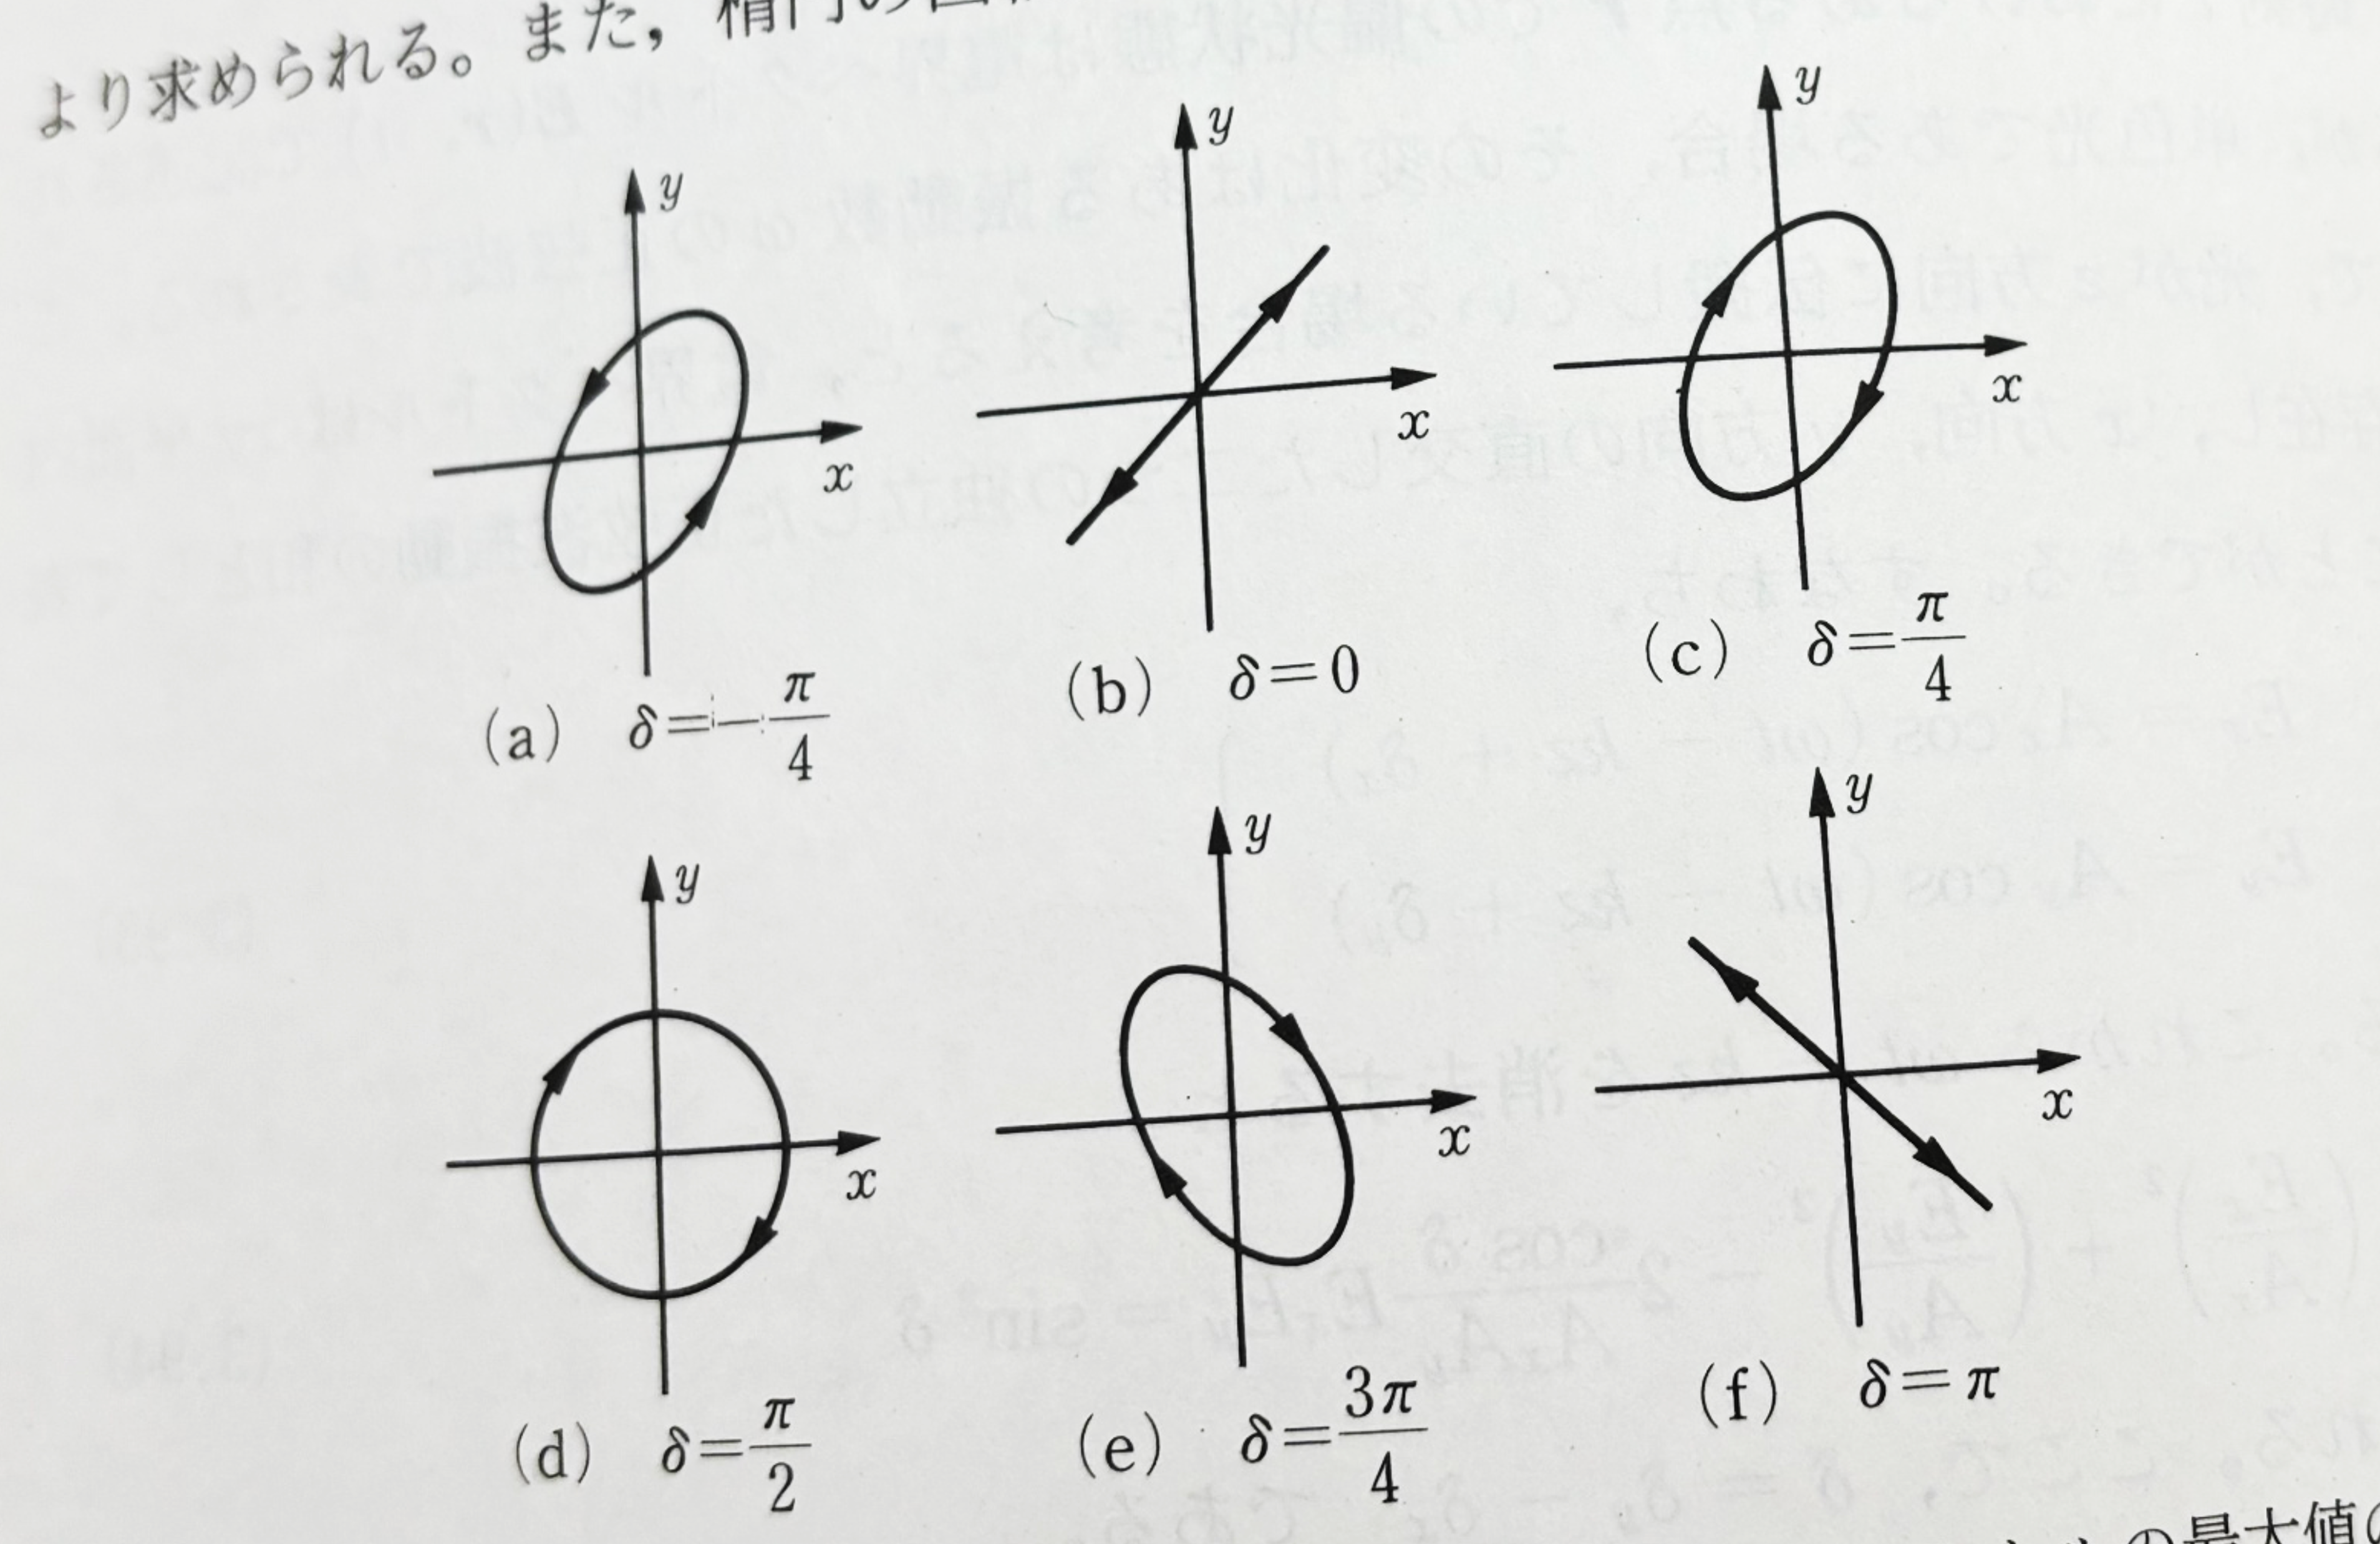
\includegraphics[width=0.92\linewidth]{appendix_1.png}
\caption{位相差$\delta$の違いによる偏光状態の変化.}
\label{fig:appendix_1}
\end{figure}


\subsubsection*{位相差(phase difference)とリタデーション(retardation)の定義}
一軸性媒質(単軸結晶や液晶補償板)では,電場は一般に互いに直交する2つの固有偏光(常光・異常光)に分解され,
それぞれ異なる屈折率で伝搬する.常光屈折率を $n_o$,異常光屈折率を $n_e$,板厚を $d$,真空波長を $\lambda$
とすると,両成分の光路差(optical path difference; OPD)は
\begin{equation}
\Delta L = (n_e-n_o)\,d \equiv \Delta n\,d
\label{eq:OPD}
\end{equation}
で与えられる.ここで $\Delta n=n_e-n_o$ を複屈折(birefringence)と呼ぶ.

\emph{リタデーション(retardation)}はこの光路差を長さとして表した量であり,文献により
$R=\Delta n\,d$(単位:長さ)として定義されることが多い:
\begin{equation}
R \equiv \Delta n\,d .
\label{eq:retardation_length}
\end{equation}
一方,Jones行列に直接現れるのは,固有偏光間に蓄積される位相差(phase difference)であり,
\begin{equation}
\Gamma
=
\frac{2\pi}{\lambda}\,R
=
\frac{2\pi}{\lambda}\,\Delta n\,d
\label{eq:phase_difference}
\end{equation}
で与えられる($\Gamma$ は無次元の位相).したがって,
\begin{itemize}
\item retardation $R$:光路差(長さ)の意味をもつ量(例:$\mathrm{nm}$)
\item phase difference $\Gamma$:位相差(角度)の意味をもつ量(例:$\mathrm{rad}$)
\end{itemize}
という区別がある.実務上は「リタデーション」と言って $\Gamma$(位相差)を指す場合もあるため,
以後は必要に応じて $R$(長さ)と $\Gamma$(位相)を明示して混同を避ける.

\subsubsection*{$\lambda/2$板と$\lambda/4$板}
位相差板は,特定波長 $\lambda$ において位相差 $\Gamma$ が所望の値となるように設計される.
代表例として
\begin{align}
\lambda/2\ \text{板(half-wave plate; HWP)}: \quad & \Gamma=\pi \quad \Leftrightarrow \quad R=\frac{\lambda}{2},
\label{eq:HWP}\\
\lambda/4\ \text{板(quarter-wave plate; QWP)}: \quad & \Gamma=\frac{\pi}{2} \quad \Leftrightarrow \quad R=\frac{\lambda}{4}
\label{eq:QWP}
\end{align}
である.ここでの $\lambda$ は設計波長であり,分散のため一般に波長がずれると $\Gamma$ もずれる.

\subsubsection*{A-plate と C-plate(液晶補償板の基本分類)}
LCDの視野角補償では,一軸性の補償板を「光学軸の向き」で分類して用いることが多い.

\begin{itemize}
\item \textbf{A-plate(uniaxial A-plate)}: 光学軸が基板面内(in-plane)にある一軸板.
例えば座標を基板法線を $z$,面内を $x,y$ とすると,光学軸が $x$ 方向($\mathbf{a}\parallel \hat{\mathbf{x}}$)
にある場合を典型とする.正入射近傍では,面内の直交成分(概ね $x$ と $y$ 成分)が
それぞれ異常光・常光に対応し,位相差を生む.

\item \textbf{C-plate(uniaxial C-plate)}: 光学軸が基板法線方向(out-of-plane)にある一軸板.
すなわち $\mathbf{a}\parallel \hat{\mathbf{z}}$.正入射では面内の任意の偏光が常光として見える(理想化)ため
位相差を生じにくいが,斜入射では有効屈折率が角度依存となり位相差が現れ,視野角補償に重要となる.
\end{itemize}

以上のように,HWP,QWPは位相差による分類であり,A-plate,C-plateは光学軸方位による分類であることに注意する.

\subsubsection*{A-plate に直線偏光が入射したときの偏光状態変換}
本節では理解を容易にするため,まず正入射近傍での単純化した議論を述べる.
波長板などは「$x$ 成分と $y$ 成分に異なる位相を与える」素子である.例えば位相差 $\Gamma$ のリターダは
\begin{equation}
\begin{pmatrix}\tilde E_x'\\ \tilde E_y'\end{pmatrix}
=
\begin{pmatrix}1&0\\0&e^{i\Gamma}\end{pmatrix}
\begin{pmatrix}\tilde E_x\\ \tilde E_y\end{pmatrix}
\label{eq:retarder_simple}
\end{equation}
と表せる.

A-plate を「主軸が $x$ に一致する位相差板」とみなし,入射偏光が主軸に対して角度 $\alpha$ をなす直線偏光
\begin{equation}
\mathbf{j}_{\mathrm{in}}
=
\begin{pmatrix}
\cos\alpha\\
\sin\alpha
\end{pmatrix}
\label{eq:lin_in_alpha}
\end{equation}
で与えられるとする.主軸基底での位相差板の作用は
\begin{equation}
\mathbf{j}_{\mathrm{out}}
=
\begin{pmatrix}
1&0\\
0&e^{i\Gamma}
\end{pmatrix}
\begin{pmatrix}
\cos\alpha\\
\sin\alpha
\end{pmatrix}
=
\begin{pmatrix}
\cos\alpha\\
e^{i\Gamma}\sin\alpha
\end{pmatrix}.
\label{eq:lin_out_alpha}
\end{equation}
ここで偏光状態を決めるのは振幅比 $\tan\alpha$ と相対位相差 $\Gamma$ である.
\\

ex.(i) $\lambda/2$板($\Gamma=\pi$)の場合:直線偏光の回転:\\
$\Gamma=\pi$ なので
\begin{equation}
\mathbf{j}_{\mathrm{out}}
=
\begin{pmatrix}
\cos\alpha\\
-\sin\alpha
\end{pmatrix}
\propto
\begin{pmatrix}
\cos(-\alpha)\\
\sin(-\alpha)
\end{pmatrix}
\label{eq:HWP_linear}
\end{equation}
となり,出射は依然として直線偏光である(位相差が $\pi$ なので符号反転に対応).
より一般には,主軸から角度 $\alpha$ の直線偏光は,$\lambda/2$板により
「主軸に関して鏡映」され,偏光方位が $2\alpha$ だけ回転した直線偏光になる.

ex.(ii) $\lambda/4$板($\Gamma=\pi/2$)の場合:直線$\to$円(条件付き):\\
$\Gamma=\pi/2$ なので
\begin{equation}
\mathbf{j}_{\mathrm{out}}
=
\begin{pmatrix}
\cos\alpha\\
i\,\sin\alpha
\end{pmatrix}.
\label{eq:QWP_general}
\end{equation}
一般の $\alpha$ では楕円偏光となるが,特に入射が主軸に対して $45^\circ$(すなわち $\alpha=\pi/4$)のとき
\begin{equation}
\mathbf{j}_{\mathrm{out}}
=
\frac{1}{\sqrt{2}}
\begin{pmatrix}
1\\
i
\end{pmatrix}
\label{eq:QWP_circular}
\end{equation}
となり,右(または規約により左)円偏光が得られる.
同様に $\alpha=-\pi/4$ では $\frac{1}{\sqrt{2}}(1,-i)^{\mathsf T}$ となり反対の円偏光となる.
従って,A-plate(位相差板)に直線偏光を入射すると,$\Gamma$ が一般値なら楕円偏光,
$\Gamma=\pi$ なら直線偏光,$\Gamma=\pi/2$ かつ $\alpha=\pm\pi/4$ の条件で円偏光が得られる.
\\

以上のように,
位相差板は固有偏光成分に\emph{位相}を付与する素子であり,個々の成分の強度(振幅)自体は変えない.
しかし,2成分間の相対位相差 $\Gamma$ が偏光楕円の形を決めるため,
「位相だけの操作」であっても一般には直線$\leftrightarrow$楕円$\leftrightarrow$円という偏光状態変換が生じる.
この点が,Jonesベクトルを複素数で表すことの物理的必然性である.

\subsection{Jones行列の一般論}
以上より,偏光状態を最小自由度で完全に表現し,かつ偏光素子の作用を線形代数的に簡潔に扱うためには, 
複素2成分のJonesベクトルが自然な選択であることが分かる. 
Jonesベクトルとその作用を以下にまとめる.
単色平面波が一様媒質中を伝搬する状況を考える.伝搬方向を $\hat{\mathbf{k}}$ とし,電場は横波条件
\begin{equation}
\mathbf{E}\cdot\hat{\mathbf{k}}=0
\label{eq:transversality}
\end{equation}
を満たす.通常のJones計算では,(正入射あるいは小角近似の下で)横波面を固定し,
その面内の直交基底 $\{\hat{\mathbf{e}}_1,\hat{\mathbf{e}}_2\}$ に関する複素振幅で偏光状態を表す.
すなわち,(空間位相因子を省略して)
\begin{equation}
\mathbf{E}(t)=\Re\Bigl\{ \bigl(E_1\,\hat{\mathbf{e}}_1 + E_2\,\hat{\mathbf{e}}_2\bigr)e^{-i\omega t}\Bigr\},
\qquad
\mathbf{j}=
\begin{pmatrix}
E_1\\
E_2
\end{pmatrix}\in\mathbb{C}^2
\label{eq:jones_vector}
\end{equation}
をJonesベクトルとする.

ここで重要なのは,観測される電場 $\mathbf{E}(t)$ は実数である一方,単色波では時間依存 $e^{-i\omega t}$ を共通因子として分離できるため,
偏光状態の情報は複素振幅(フェーザ)$E_1,E_2$ に集約できる点である.すなわち
\begin{equation}
E_1=A_1 e^{i\phi_1},\qquad E_2=A_2 e^{i\phi_2}
\end{equation}
と書け,偏光楕円を規定する振幅比 $A_2/A_1$ と相対位相差 $\delta=\phi_2-\phi_1$ を自然に保持できる.
特に相対位相差 $\delta$ は円偏光・楕円偏光(例えば $\mathbf{j}\propto (1,\pm i)^{\mathsf T}$)の記述に不可欠であり,
成分を実数に限定すると一般の偏光状態を最小自由度で表せない.
実電場は式\eqref{eq:jones_vector}のとおり最終的に実部 $\Re\{\cdot\}$ を取ることで得られ,複素表示は計算上の表現である.

\subsection{一様媒質内の偏光の伝搬}
横波条件\eqref{eq:transversality}により電場は光の伝搬方向 $\hat{\mathbf{k}}$ に直交する2次元部分空間に属する.
そのため,媒質が光の伝搬方向 $\hat{\mathbf{k}}$ に垂直に配置
されている場合には,
横波面内の直交基底 $\{\hat{\mathbf{e}}_1,\hat{\mathbf{e}}_2\}$ を選べば偏光状態は2成分で完全に表現できる.
この「2成分(横波面)+複素数(振幅と位相)」という最小表現を採用することで,
位相遅れ素子が成分に位相因子 $e^{i\Gamma}$ を掛ける操作として記述され,偏光光学素子を線形変換として扱える.

線形・時間不変な偏光光学素子は $2\times 2$ 複素行列 $M\in\mathbb{C}^{2\times 2}$ により
\begin{equation}
\mathbf{j}_{\mathrm{out}}=M\,\mathbf{j}_{\mathrm{in}}
\label{eq:jones_action}
\end{equation}
と記述され,直列素子の合成は行列積で与えられる.複素2成分を用いることにより,
(例えば位相差板のような)位相の付与が乗算として線形に表され,計算が簡潔に保たれる.

主軸基底で位相差 $\Gamma$ を与える理想リターダは
\begin{equation}
J(\Gamma)=
\begin{pmatrix}
e^{+i\Gamma/2} & 0\\
0 & e^{-i\Gamma/2}
\end{pmatrix},
\label{eq:retarder}
\end{equation}
主軸が基底 $\{\hat{\mathbf{e}}_1,\hat{\mathbf{e}}_2\}$ に対して角度 $\theta$ だけ回転している場合は
\begin{equation}
M_{\mathrm{ret}}(\theta,\Gamma)=R(-\theta)\,J(\Gamma)\,R(\theta)
\label{eq:retarder_rotated}
\end{equation}
と書ける.ここで $R(\theta)\in\mathbb{R}^{2\times 2}$ は2次元回転行列
\begin{equation}
R(\theta)=
\begin{pmatrix}
\cos\theta & -\sin\theta\\
\sin\theta & \cos\theta
\end{pmatrix},
\qquad
R^{\mathsf T}R=I_2,\ \det R=+1
\label{eq:R_def}
\end{equation}
である.重要なのは,\eqref{eq:retarder_rotated} は
\emph{同一の2次元横波面(同一のJones空間)内での基底変換}として完結しており,斜入射に伴う横波面の回転や,
界面におけるFresnel係数の偏光依存($t_s\neq t_p$)等は基本的に含まれない点である.

% --- ここを「\subsubsection{Conventional Jones calculus ...}」(=0.1.1節) の直後に挿入 ---


\subsection{例:一軸位相差板をクロスニコル(直交偏光板)で挟んだ透過強度}
\label{sec:example_crossed_nicols}

\begin{figure}[htb]
\centering
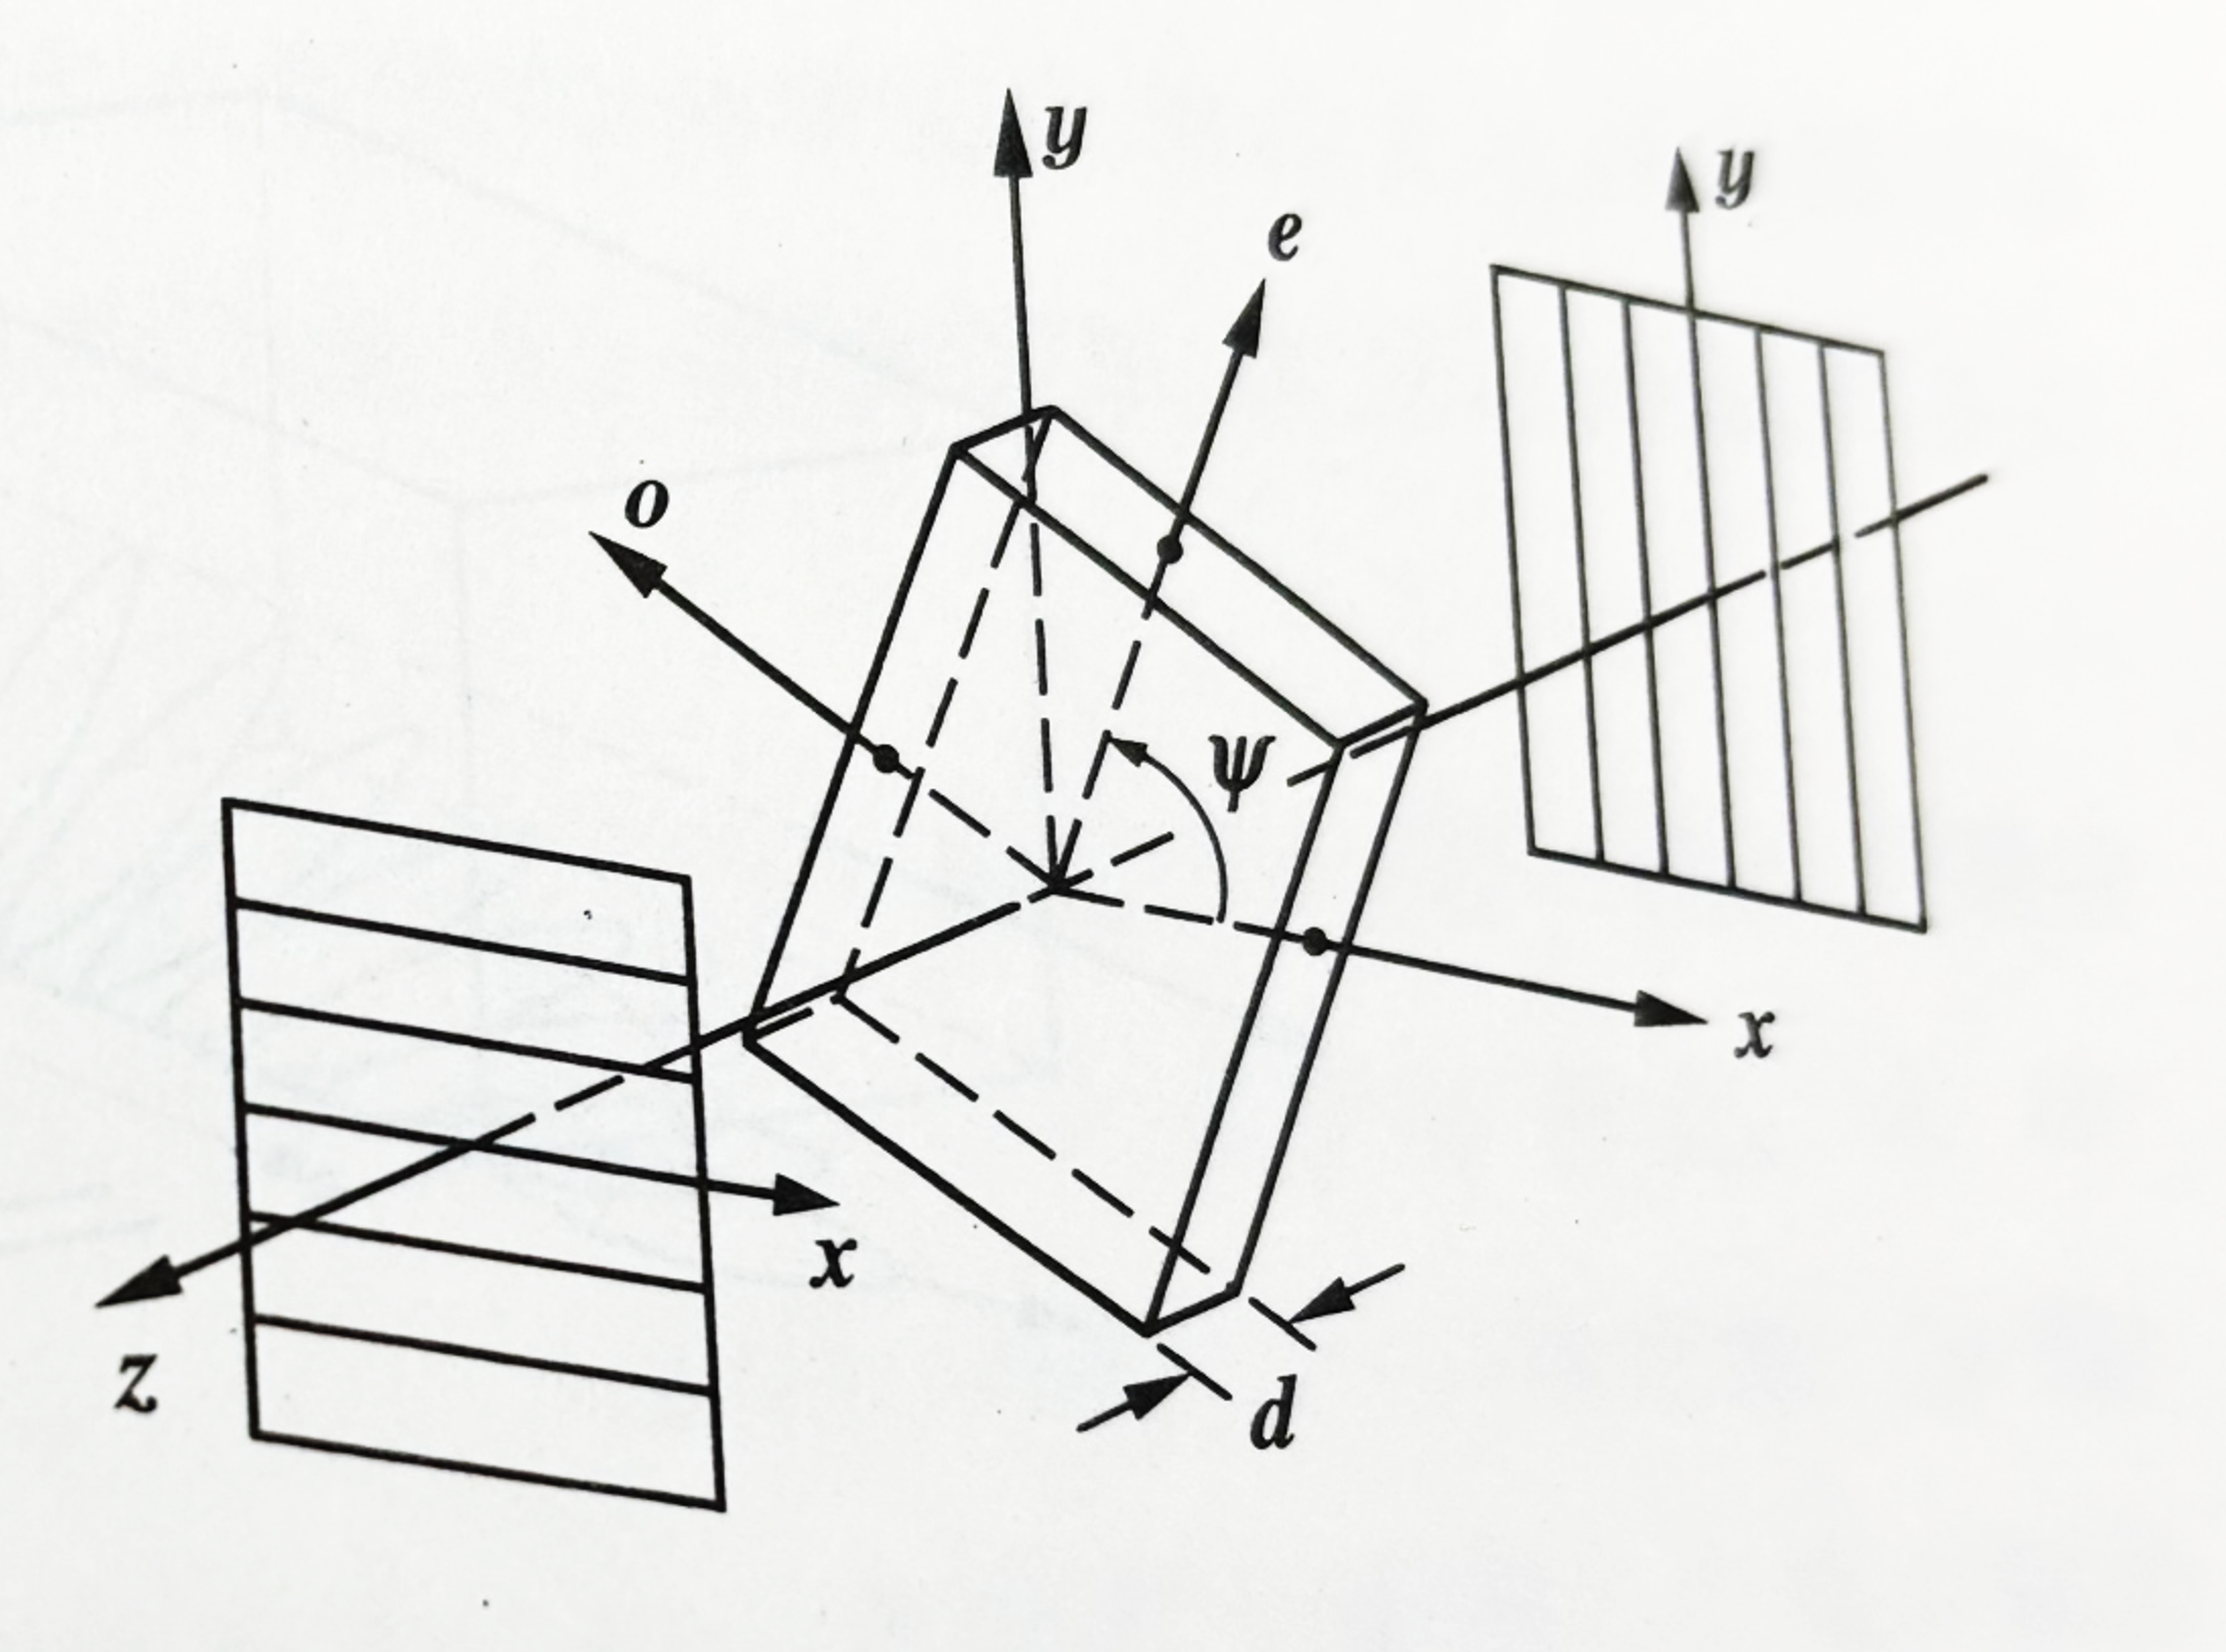
\includegraphics[width=0.92\linewidth]{appendix_2.png}
\caption{一軸位相差板をクロスニコル偏光板で挟んだ場合の光の伝搬.}
\label{fig:appendix_2}
\end{figure}

ここでは通常のJones計算の代表例として,透過軸が互いに直交する2枚の偏光板(クロスニコル)で
一軸の理想位相差板(リターダ)を挟んだ場合の出射光強度を導出する.
構成を図\ref{fig:appendix_2}に示す.

本文との整合のため,本節では偏光板を明示的なJones行列として挿入せず,
入射側偏光板は「入射偏光(透過後状態)の設定」,出射側偏光板(Analyzer)は「Analyzerの透過状態への射影」として扱う.
すなわち,入射側偏光板の透過状態を $\mathbf{o}_1$,解析器の透過状態を $\mathbf{o}_2$ とし,
層(ここでは位相差板)の作用素を $M$ とすると,透過振幅 $a$ と強度 $I_\perp$ は
\begin{equation}
a=\mathbf{o}_2^{\mathsf T} M\,\mathbf{o}_1\,E_0,
\qquad
I_\perp \propto |a|^2
\label{eq:main_form_amplitude}
\end{equation}
で与えられる.

以下,Jones基底を $(x,y)$ とし,入射側偏光板は $x$ 透過,Analyzerは $y$ 透過(クロスニコル条件)とする.
したがって許容状態は
\begin{equation}
\mathbf{o}_1=
\begin{pmatrix}
1\\
0
\end{pmatrix},
\qquad
\mathbf{o}_2=
\begin{pmatrix}
0\\
1
\end{pmatrix}
\label{eq:o1o2_xy}
\end{equation}
である(ここでは2次元表記を用いる).

位相差板は,主軸基底での位相差(retardation)を $\Gamma$ とし,
\eqref{eq:retarder} の $J(\Gamma)$ により表す.
主軸が入射偏光板の透過軸($x$)から角度 $\theta$ だけ回転しているとき,位相差板のJones行列は
\eqref{eq:retarder_rotated} により
\begin{equation}
M_{\mathrm{ret}}(\theta,\Gamma)=R(-\theta)\,J(\Gamma)\,R(\theta)
\label{eq:Mret_again}
\end{equation}
である.

入射光は入射偏光板を通過した $x$ 直線偏光(振幅 $E_0$)として与える:
\begin{equation}
\mathbf{j}_{\mathrm{in}}
=
E_0\,\mathbf{o}_1
=
\begin{pmatrix}
E_0\\
0
\end{pmatrix}.
\label{eq:jin_xpol}
\end{equation}
このとき,解析器透過成分の振幅は
\begin{equation}
a
=
\mathbf{o}_2^{\mathsf T} \,M_{\mathrm{ret}}(\theta,\Gamma)\,\mathbf{j}_{\mathrm{in}}
=
E_0\,\mathbf{o}_2^{\mathsf T} \,M_{\mathrm{ret}}(\theta,\Gamma)\,\mathbf{o}_1
\label{eq:a_def}
\end{equation}
で与えられる.すなわち本節は,明示的な偏光板行列を用いず
(入射側は初期条件,出射側は射影として)透過強度を求める計算例になっている.

\eqref{eq:Mret_again} を用いて $a$ を計算すると,
\begin{align}
\mathbf{o}_2^{\mathsf T}M_{\mathrm{ret}}(\theta,\Gamma)\mathbf{o}_1
&=
\begin{pmatrix}0&1\end{pmatrix}
R(-\theta)\,J(\Gamma)\,R(\theta)
\begin{pmatrix}1\\0\end{pmatrix}
\nonumber\\
&=
\frac{1}{2}\sin(2\theta)\Bigl(e^{+i\Gamma/2}-e^{-i\Gamma/2}\Bigr)
=
i\,\sin(2\theta)\,\sin\!\left(\frac{\Gamma}{2}\right),
\label{eq:a_over_E0}
\end{align}
(位相因子 $i$ は強度には寄与しない).
したがって
\begin{equation}
a
=
iE_0\,\sin(2\theta)\,\sin\!\left(\frac{\Gamma}{2}\right),
\label{eq:Ey_out}
\end{equation}
となり,透過強度は
\begin{equation}
I_{\perp}
\;\propto\;
|a|^2
=
|E_0|^2\,\sin^2(2\theta)\,\sin^2\!\left(\frac{\Gamma}{2}\right).
\label{eq:I_crossed_retarder}
\end{equation}
入射強度 $I_0\propto |E_0|^2$ を用いれば
\begin{equation}
\frac{I_{\perp}}{I_0}
=
\sin^2(2\theta)\,\sin^2\!\left(\frac{\Gamma}{2}\right)
\label{eq:Iratio_crossed_retarder}
\end{equation}
が得られる.これはクロスニコル間に挿入した位相差板の標準結果であり,
透過が(i)主軸方位 $\theta$ と(ii)位相差 $\Gamma$ の両方で制御されることを示す.

\subsection{式\eqref{eq:Iratio_crossed_retarder}に基づくIPSの暗状態・明状態の解釈}
\label{sec:IPS_dark_bright_from_crossed}

IPS(In-Plane Switching)では,電圧印加により液晶ディレクタ(有効光学軸)が基板面内で回転し,
光学軸方位角が $\phi(V)$ として変化する(面内回転が主効果)とみなせる.
正入射近傍では,液晶層は「一軸位相差板」として近似でき,
その有効位相差を $\Gamma(V)$,偏光板透過軸に対する主軸角を
\begin{equation}
\theta(V)=\phi(V)-\phi_{\mathrm{pol}}
\label{eq:theta_of_V}
\end{equation}
とおけば,クロスニコル構成における透過は
\begin{equation}
\frac{I_{\perp}(V)}{I_0}
=
\sin^2\!\bigl(2\theta(V)\bigr)\,
\sin^2\!\left(\frac{\Gamma(V)}{2}\right)
\label{eq:Iratio_IPS_simple}
\end{equation}
で表される.

\textbf{暗状態(Normally Black の基本像)}:
IPSの代表的な動作は「オフで暗,オンで明」である.
クロスニコル構成で $V=0$ のときディレクタが偏光板透過軸に整列していれば
\begin{equation}
\theta(0)\approx 0 \quad (\text{または } \pi/2)
\end{equation}
となり,
\begin{equation}
\sin^2\!\bigl(2\theta(0)\bigr)\approx 0
\quad\Rightarrow\quad
I_{\perp}(0)\approx 0
\label{eq:dark_condition}
\end{equation}
が得られる.すなわち暗状態は主に「面内方位がクロス条件を満たす」ことにより実現される.

\textbf{明状態(オンで透過を最大化)}:
電圧を印加してディレクタが面内で回転し,
\begin{equation}
\theta(V)\to \frac{\pi}{4}
\label{eq:bright_angle}
\end{equation}
に近づくと,$\sin^2(2\theta)$ が最大(=1)となり,
\begin{equation}
\frac{I_{\perp}(V)}{I_0}\approx \sin^2\!\left(\frac{\Gamma(V)}{2}\right)
\label{eq:bright_limited_by_Gamma}
\end{equation}
まで透過が増大する.従って明状態の上限は位相差 $\Gamma(V)$ により規定される.
特に
\begin{equation}
\Gamma(V)\approx \pi \quad (\text{半波条件})
\end{equation}
が満たされる波長では $\sin^2(\Gamma/2)\approx 1$ となり高透過が得られる.
一方,$\Gamma$ は波長依存性(分散)と厚み・複屈折に依存するため,
実際のIPSでは補償膜等により視野角・波長での最適化が行われる.

以上より,式\eqref{eq:Iratio_IPS_simple}の観点からは,
IPSの暗・明状態は次の二つの因子に分離して理解できる:
\begin{enumerate}
\item 面内回転による主軸角 $\theta(V)$ の制御(幾何学因子 $\sin^2(2\theta)$)
\item 層の有効位相差 $\Gamma(V)$ の制御(位相因子 $\sin^2(\Gamma/2)$)
\end{enumerate}
IPSでは主として (1) が変調の主因であり,
(2) は波長・視野角・材料定数・厚みで決まる設計パラメータとして透過上限や色特性を支配する,
という整理が得られる.


\section{斜入射における偏光伝搬の取り扱い}
\label{app:oblique_main_method}

本付録では,視線方向が法線から傾いた斜入射(oblique incidence)における偏光伝搬を,
本文で用いた光の進行方向に垂直な「横波面(transverse plane)平面上の2成分Jones作用を3次元空間へ埋め込む」枠組みとして整理する.
この定式化は,層を理想リターダ(位相差素子)として扱いながら,
斜入射で本質となる横波条件と基底の幾何学を明示的に取り込むことを目的とする.
最後に,界面のFresnel効果を明示的に含む拡張Jones(Extended Jones)法との相違点をまとめる.

\subsection{幾何学的準備:横波条件と横波面射影}
\label{app:geom_transverse}

単色平面波の伝搬方向を単位ベクトル $\hat{\mathbf{k}}=\hat{\mathbf{k}}(\theta,\phi)$ とする.
電場 $\mathbf{E}$ は横波条件
\begin{equation}
\mathbf{E}\cdot\hat{\mathbf{k}}=0
\label{eq:app_transversality}
\end{equation}
を満たし,したがって $\mathbf{E}$ は $\hat{\mathbf{k}}$ に直交する2次元部分空間
\begin{equation}
\mathcal{T}(\hat{\mathbf{k}})=\{\mathbf{v}\in\mathbb{R}^3\mid \mathbf{v}\cdot\hat{\mathbf{k}}=0\}
\end{equation}
(横波面)に属する.任意の3次元ベクトルを横波面へ射影する直交射影行列を
\begin{equation}
P_\perp(\hat{\mathbf{k}})=I_3-\hat{\mathbf{k}}\hat{\mathbf{k}}^{\mathsf T}
\label{eq:app_Pperp}
\end{equation}
と定義する.数値計算では層を跨ぐ演算により縦成分($\parallel \hat{\mathbf{k}}$)が微小に混入することがあるため,
必要に応じて $P_\perp$ を適用して横波条件\eqref{eq:app_transversality}を保つ.

\subsection{偏光板の扱い}
\label{app:polarizer_state}

本手法では,入射偏光板および出射偏光板 (Analyzer)を明示的なJones行列 $P$ として挿入せず,
各視線方向 $\hat{\mathbf{k}}$ に対する偏光板の\emph{有効透過偏光状態}ベクトルを導入して扱う.

偏光板の吸収軸(あるいは偏光板の姿勢を規定する参照軸)を3次元ベクトル $\mathbf{c}$ で与えるとき,
視線方向 $\hat{\mathbf{k}}$ に対して横波条件を満たす偏光板の(off-axis)有効透過軸ベクトルを
\begin{equation}
\mathbf{o}(\hat{\mathbf{k}},\mathbf{c})
=
\frac{\hat{\mathbf{k}}\times \mathbf{c}}{\|\hat{\mathbf{k}}\times \mathbf{c}\|}
\label{eq:app_o_def}
\end{equation}
により定義する($\hat{\mathbf{k}}\times\mathbf{c}\neq \mathbf{0}$ を仮定).
この $\mathbf{o}(\hat{\mathbf{k}},\mathbf{c})$ は単位ベクトルであり,$\mathbf{o}\cdot\hat{\mathbf{k}}=0$ を満たすため,
横波面内の1次元透過モード(=透過状態)を与える.

入射側偏光板の有効透過状態を $\mathbf{o}_1=\mathbf{o}(\hat{\mathbf{k}},\mathbf{c}_1)$,
解析器(analyzer)の有効透過状態を $\mathbf{o}_2=\mathbf{o}(\hat{\mathbf{k}},\mathbf{c}_2)$ とすると,
入射電場は偏光板通過後の状態として
\begin{equation}
\mathbf{E}_{\mathrm{in}} = E_0\,\mathbf{o}_1
\label{eq:app_Ein}
\end{equation}
と与えることができる.出射側では解析器の透過状態への射影により透過振幅を定義し,
\begin{equation}
a=\mathbf{o}_2^{\mathsf T}\mathbf{E}_{\mathrm{out}},\qquad
I\propto |a|^2
\label{eq:app_analyzer_projection}
\end{equation}
として透過強度を評価する.

なお,理想偏光板を3次元射影作用行列(正入射近傍では横波面上の $2\times2$ Jones行列に対応する表現)で表すなら
\begin{equation}
P^{(3D)}(\hat{\mathbf{k}})=\mathbf{o}(\hat{\mathbf{k}},\mathbf{c})\,\mathbf{o}(\hat{\mathbf{k}},\mathbf{c})^{\mathsf T}
\end{equation}
であり,上記の取り扱いはこれと等価である.ただし本手法では,
入射側偏光板の作用を入射偏光状態\eqref{eq:app_Ein}に吸収し,
出射側は射影\eqref{eq:app_analyzer_projection}で透過成分を直接読み出す点に特徴がある.

\subsection{層の記述:横波面基底と埋め込み行列 $U_n$}
\label{app:Un_def}

層 $n$ を3次元の光学軸(単位ベクトル)$\mathbf{a}_n$ と位相差(retardation)$\Gamma_n$ で記述する.
与えられた視線方向 $\hat{\mathbf{k}}$ に対し,光学軸の横波面への射影
\begin{equation}
\mathbf{a}_{n,\perp}=P_\perp(\hat{\mathbf{k}})\mathbf{a}_n
=\mathbf{a}_n-(\mathbf{a}_n\cdot\hat{\mathbf{k}})\hat{\mathbf{k}}
\label{eq:app_axis_projection}
\end{equation}
を計算し,$\|\mathbf{a}_{n,\perp}\|\neq 0$ のとき横波面正規直交基底を
\begin{equation}
\mathbf{u}_n=\frac{\mathbf{a}_{n,\perp}}{\|\mathbf{a}_{n,\perp}\|},
\qquad
\mathbf{v}_n=\hat{\mathbf{k}}\times\mathbf{u}_n
\label{eq:app_uv_def}
\end{equation}
により定める($\mathbf{a}_n\parallel\hat{\mathbf{k}}$ の特異点では任意の横波面基底を選べばよい).
このとき埋め込み行列
\begin{equation}
U_n=\begin{pmatrix}\mathbf{u}_n & \mathbf{v}_n\end{pmatrix}\in\mathbb{R}^{3\times 2}
\label{eq:app_Un}
\end{equation}
は
\begin{equation}
U_n^{\mathsf T}U_n=I_2,\qquad
U_nU_n^{\mathsf T}=P_\perp(\hat{\mathbf{k}})
\label{eq:app_U_properties}
\end{equation}
を満たし,横波面の2成分表現と偏光の3次元空間上の電場を厳密に接続する.

\subsection{層作用素:2次元Jones作用の3次元への埋め込み}
\label{app:Mn_def}

横波面基底 $(\mathbf{u}_n,\mathbf{v}_n)$ 上で,層 $n$ を位相差 $\Gamma_n$ の理想リターダとして扱うと,
2次元Jones行列は
\begin{equation}
J_n(\Gamma_n)=
\begin{pmatrix}
e^{+i\Gamma_n/2} & 0\\
0 & e^{-i\Gamma_n/2}
\end{pmatrix}
\label{eq:app_Jn}
\end{equation}
で与えられる.これを3次元空間内に埋め込む操作が
\begin{equation}
M_n(\hat{\mathbf{k}};\mathbf{a}_n,\Gamma_n)=U_n\,J_n(\Gamma_n)\,U_n^{\mathsf T}
\label{eq:app_Mn}
\end{equation}
である.

\subsection{多層スタックと透過強度}
\label{app:stack_intensity}

層が $n=1,\dots,N$ の順に直列に並ぶとき,全体作用素を
\begin{equation}
M_{\mathrm{stack}}(\hat{\mathbf{k}})
=
\prod_{n=1}^{N} M_n(\hat{\mathbf{k}};\mathbf{a}_n,\Gamma_n)
\label{eq:app_stack}
\end{equation}
(右端が入射側,左端が出射側:順序は本文の定義に従う)として,
\begin{equation}
\mathbf{E}_{\mathrm{out}} = M_{\mathrm{stack}}(\hat{\mathbf{k}})\,\mathbf{E}_{\mathrm{in}}
= E_0\,M_{\mathrm{stack}}(\hat{\mathbf{k}})\,\mathbf{o}_1
\label{eq:app_Eout}
\end{equation}
を得る.解析器透過振幅と強度は
\begin{equation}
a(\hat{\mathbf{k}})=\mathbf{o}_2^{\mathsf T} \mathbf{E}_{\mathrm{out}}
=E_0\,\mathbf{o}_2^{\mathsf T} M_{\mathrm{stack}}(\hat{\mathbf{k}})\mathbf{o}_1,
\qquad
I(\hat{\mathbf{k}})\propto |a(\hat{\mathbf{k}})|^2
\label{eq:app_I}
\end{equation}
で与えられる.暗状態漏れや視野角特性は $I(\theta,\phi)$ を走査して評価する.

以上のように,本手法は,斜入射問題における本質的困難の一つである「横波面の回転」と「基底の選び方」を
$U_n$ と $\mathbf{o}(\hat{\mathbf{k}},\mathbf{c})$ により幾何学的に明示した上で,
層を位相差 $\Gamma_n$ の理想リターダとして表現する枠組みである.
従って,層内部の吸収や散乱,および界面でのFresnel係数の偏光依存($t_s\neq t_p$)や
異方性界面に起因する偏光混合は,基本形では陽に含まれない.

\subsection{拡張Jones(Extended Jones)法との相違点}
\label{app:diff_extended_jones}

\subsubsection{Extended Jones 法の要点(概念)}
\label{app:extj_summary}

Extended Jones 法(Gu--Yeh 型)は,斜入射で通常Jonesが破綻する主因である界面効果を
2成分表現の中に取り込むことを目的とする.外部媒質で定義した $s/p$ 成分振幅
$(A_s,A_p)^{\mathsf T}$ を状態変数とし,単一一軸板の透過を典型的に
\begin{equation}
\begin{pmatrix}A_s'\\A_p'\end{pmatrix}
=
D_o\,P\,D_i
\begin{pmatrix}A_s\\A_p\end{pmatrix}
\label{eq:app_extj_form}
\end{equation}
と表す.ここで $P$ は板内部固有モード($o/e$)の伝搬位相(対角行列),
$D_i, D_o$ は入射・出射界面でのモード分解・再合成とFresnel透過係数を含む「dynamical matrix」であり,
一般に回転行列ではない(振幅差 $t_s\neq t_p$ や結合を含み得る).
多重反射を無視する近似を置くことが多い一方,単回の界面条件は陽に保持される.

\subsubsection{相違点の整理}
\label{app:diff_points}

本手法(main.pdf)と Extended Jones 法の差異は,主に「界面をどこまでモデルに含めるか」に集約される.
以下に要点をまとめる.

\begin{enumerate}
\item \textbf{状態変数(2成分)の定義} \\
本手法は3次元電場 $\mathbf{E}$ を基本変数とし,横波面基底を介して2成分Jones作用を埋め込む.
偏光板も $\mathbf{o}(\hat{\mathbf{k}},\mathbf{c})$ により有効透過偏光状態として与える.
一方 Extended Jones は外部媒質で定義される $s/p$ 成分 $(A_s,A_p)$ を基本変数とし,
界面条件によりそれらが混合し得ることを前提に2$\times$2を構成する.

\item \textbf{界面(Fresnel)効果の扱い} \\
本手法の基本形では,層は理想リターダ(位相差のみ)として表され,
界面での偏光依存透過($t_s\neq t_p$)や偏光混合を陽には含めない.
Extended Jones は $D_i,D_o$ により界面のFresnel係数とモード結合を明示的に含むため,
高NAや屈折率ミスマッチが大きい場合に精度向上が期待できる.

\item \textbf{幾何学(横波面回転)の取り込み方} \\
本手法は $\hat{\mathbf{k}}$ に依存する横波面を $U_n$ と $P_\perp$ により明示し,
「横波条件を保ったまま層の位相差作用を積で追跡する」ことに重点を置く.
Extended Jones では横波面の幾何は主として $s/p$ 定義(入射面)に埋め込まれ,
界面行列 $D$ の中に幾何と境界条件が統合される.

\item \textbf{計算量と設計最適化への適性} \\
本手法は $M_n=U_n J_n U_n^{\mathsf T}$ の積として実装でき,幾何学的で見通しが良く高速であるため,
補償板パラメータ($\Gamma_n$,軸方位)の最適化に適する.
Extended Jones は界面ごとに dynamical matrix を構築するため bookkeeping が増えるが,
界面支配的な漏れや視野角劣化をより忠実に扱える.

\item \textbf{適用領域の指針} \\
本手法は「漏れの主因が横波面幾何と位相差の組合せ」で説明できる領域で有効である.
一方,界面の偏光依存透過・結合が支配的となる条件(高視野角,屈折率差が大きい,多界面)では,
Extended Jones の導入が有利となる.
\end{enumerate}

\subsubsection{まとめ}
\label{app:conclusion}

本手法は,斜入射における横波面の幾何学を明示した上で,
層を位相差 $\Gamma_n$ の理想リターダとして扱う「横波面埋め込み型」定式化である.
これにより,通常Jonesの簡潔さ(行列積)を保ちながら,
斜入射で無視できない基底の回転と偏光板の有効透過状態を自然に取り込むことができる.
一方,界面のFresnel効果や偏光混合を陽に含む必要がある場合には,
Extended Jones(dynamical matrix)型の枠組みが有効である.

\end{document}
